\section{Overview}
\label{sec:FIRST_overview}

Our application is designed as a web application consisting of four main parts: the front-end, back-end, AI model server, and databases (Figure \ref{fig:Retrieval_architecture}). We choose to build a web application instead of a native one because it better supports the separation of each component over the network and hence, easier development and deployment. The components communicate via APIs over HTTP/HTTPS protocols, therefore they can be either on the same machine, on a different machine, or even on a cluster of multiple nodes. Although this greatly pile up the tech stack and hence make it much more challenging, it shows our seriousness in developing a system that is similar to real-world systems, where it comprises of many pieces and each part requires an expert in that field (e.g., database, front-end developer, etc.) to develop.

\begin{figure}[ht]
    \centering
    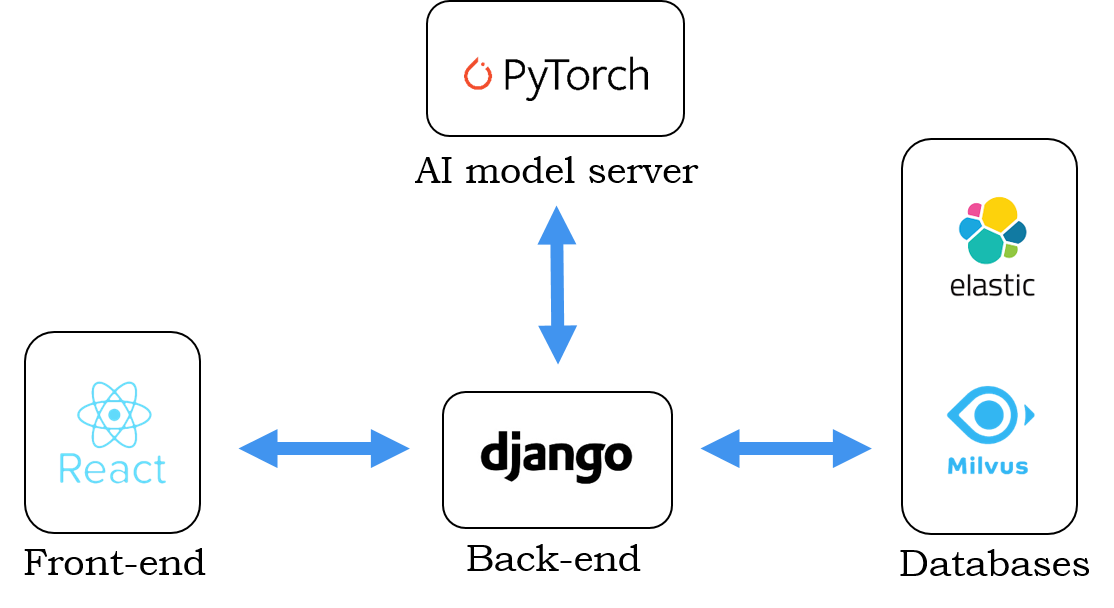
\includegraphics[width=\textwidth]{content/resources/images/methods/architecture.png}
    \caption{The architecture of our application.}
    \label{fig:Retrieval_architecture}
\end{figure}

\section{System design}
\label{sec:first_system_design}

\vspace{-2mm}
We discuss our design principles and highlight some design choices that best express said principles. These principles arise from the motivations discussed earlier in Section \ref{sec:motivation}.

\begin{itemize}
\vspace{-2mm}
    \item \textbf{Flexiblity} \quad As it is present in our system's name, flexibility is the ability to be easily altered depending on the circumstances. This is important to our objective of being a smart system, as it allows countless use cases with the correct modification. For example, using a domain-specific AI model will enable the application to work on that particular domain. To achieve this principle, we have to be clever in architecting our system such that the components are appropriately \textbf{decoupled} in order to allow modifications in functionalities as in the previous example.
\vspace{-2mm}    
    \item \textbf{Scalability} \quad We wish to work with large quantity of data, therefore scalability is essential. It is even more so because we are creating an application, where user experience can be negatively affected with just a slight increase in processing time. To realize this, we need to look beyond everyday AI model development thoughts and borrow ideas from other disciplines, such as software engineering, where there is substantial experience working with applications for the average user.
\vspace{-2mm}    
    \item \textbf{Openness} \quad Though we want our system to have a wide range of features, it cannot be omnipotent and, therefore, will have some areas that it is lacking. To address this, we propose the idea that our system does not compete with other systems, but coexist with them and acts as a complement to each other. For example, while Google does not act on user data, its cosmic knowledge base can be used to find definitions and examples of rare concepts that, in turn, can be used as the starting point for searching in our system.
\end{itemize}

\vspace{-2mm}
We note that these principles do not work in solitary. In fact, improving one can positively affect another. One notable example is that improving flexibility will lead to increased scalability, because when the system is simplified and aptly modularized, it is also easier to scale those components. We have made some design choices that reflect the principles above:

\begin{itemize}
\vspace{-2mm}
    \item \textbf{Separate visual and textual encoders}: Tackling our retrieval problem requires understanding both visual and linguistic modalities. In recent years, encoder-decoder architecture has become popularized, with Transformers\cite{vaswani_attention_2017} architecture dominating in both components. The Transformer architecture contains the multi-head attention mechanism, allowing the model to attend to different input parts. When working with multiple modalities, different works have different approaches when it comes to designing the attention head. Some approaches propose concatenating the visual and textual features and performing attention as if it were a single sequence. This gives good benchmarks results but carries a hidden computational burden at inference time.
    
\vspace{-2mm}    
    We adopt separate visual and textual encoders, which perform attention on each modality separately. The features are mapped into the same subspace, therefore we can calculate their distance as cosine distance. Computing cosine distance is factorizable, therefore we can compute the features beforehand, store them, and perform rapid computation of distances in real-time using vector databases, detailed in the following design choice. In our opinion, the benefit of significantly improving modularity far outweighs the gain in accuracy in this particular case. Furthermore, the accuracy improvement can be regained by using the simple model as a broad filter and then applying the said architecture to a smaller list of candidates.
    
\vspace{-2mm}    
    \item \textbf{Adoption of vector database}: In order to query data efficiently, a compact representation of the data is usually stored and indexed in lieu of the original data. This is a common practice for text-based data, for which various analyzers and indexes exist. However, visual data is often much larger and much more challenging to infer the semantics due to the large domain gap of the underlying representation. For this purpose, artificial intelligence and computer vision have made substantial efforts to create visual features that are much more compact and usable for searching. Nowadays, deep learning models usually embed the image into a smaller subspace (e.g., $1 * 768$) that satisfies the aforementioned needs. However, as these embeddings do not carry explicit meaning on their own (i.e., they are just a vector of floats), it is improbable to index them in ordinary databases. Therefore, vector databases have been created to enable the storage and fast query of vectors based on cosine distance.
    
\vspace{-2mm}    
    In our system, we use Milvus, a vector database that can query millions of vectors in under 100ms (based on our computational resource). To the best of our knowledge, we are among the first team to adopt this for the challenge. Milvus's performance increase is based on technology such as Facebook's FAISS, CPU-specific instructions, GPU acceleration, and more. They are necessary for good performance, yet tedious to implement from scratch. On a higher level, they also implement algorithms such as k-nearest neighbours and quantization-based inverted indexes, which are more suitable for visual data. By leveraging an existing system, we avoid having to implement these features (as many other teams do) while still using the optimal technology for the problem.
    % \item
\end{itemize}

\section{Front-end design}
\label{sec:first_front_end_design}

\vspace{-2mm}
To summarize, our front-end has the following main features:

\begin{enumerate}
\vspace{-2mm}
    \item \textbf{Web application using React}. With this separation of concern, we avoid the widespread problem of AI applications with poor user interfaces (or none at all). The front-end interacts with the back-end via APIs and the web application can be developed without knowledge of the underlying model.
\vspace{-2mm}    
    \item \textbf{Highly optimized for image viewing}. Since our main interfaces are galleries of potentially up to thousands of images, without proper optimization, it is impossible to render them. Slow rendering will prohibit fast searching, therefore we have to reduce the latency as well. To alleviate this problem, we apply a variety of techniques, including pagination, lazy loading, image compression, loading from local storage, and more.
\vspace{-2mm}    
    \item \textbf{Novel Timeline View feature}. In the previous feature, we addressed the \textit{feasibility} of displaying multiple images. However, we also need to consider its \textit{practicality}, i.e., whether the user can gain information by looking at multiple images in succession. We propose a feature that lets the user view a sequence of images with varying levels of detail based on their need. This feature is discussed in detail in Section \ref{sec:timeline_view}.
\end{enumerate}

\subsection{User interface}

\subsubsection{Main search interface}

Our primary search interface is depicted in Figure \ref{fig:FIRST_mainpage}. It consists of the search bar, which is located at the top, the gallery, which makes up most of the interface, and some other auxiliary elements. The gallery shows search results in decreasing order of relevance, from up to bottom, left to right, with the most relevant item at the top left.

\begin{figure}[h]
    \centering
    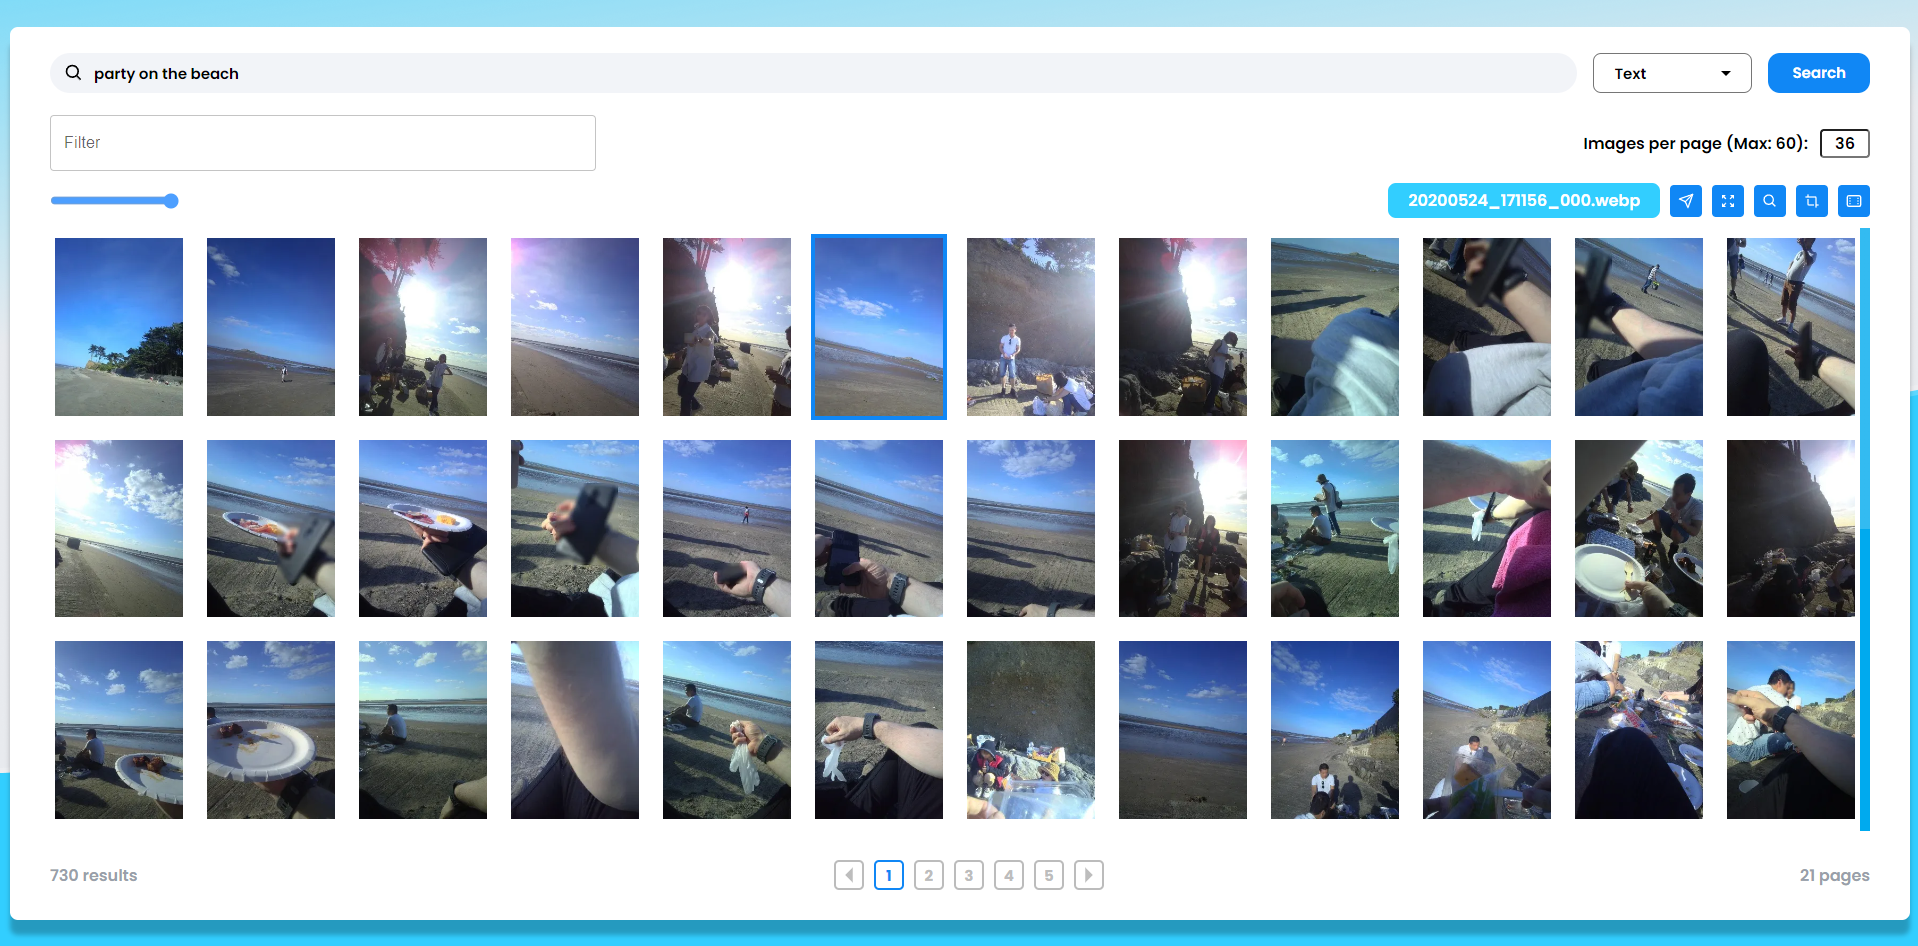
\includegraphics[width=\textwidth]{content/resources/images/methods/FIRST_mainpage.png}
    \caption{The main searching interface of our system.}
    \label{fig:FIRST_mainpage}
\end{figure}

\subsubsection{Timeline View}
\label{sec:timeline_view}

When the user selects an image and chooses the Timeline View function, they will be shown all the images on the same day or in the same video, depending on the use case. The purpose of this function is to allow fast browsing in chronological order to retrieve events that occur before and after a moment. Therefore, when the user switches to Timeline View, which has a gallery view similar to the main interface, there is a button that will quickly scroll to the selected image. If the user wants to look at the image closely, they can switch to Single image mode, which will bring the current image to the middle of the screen and leave only a slider at the bottom. This slider is another way to quickly browse in the time dimension, inspired by the YouTube slider.

Our most notable feature is that we speed up the process of viewing a sequence of images by allowing users to view it with \textbf{varying level of details}. The user can choose to \textit{decrease} the level of detail to quickly find the segment they are looking for, then they can opt to \textit{increase} the level of detail to locate the correct image at \textbf{singe frame precision}. The inner workings of this feature are disclosed in Section \ref{sec:temporal_navigation}.

\begin{figure}[H]
    \centering
    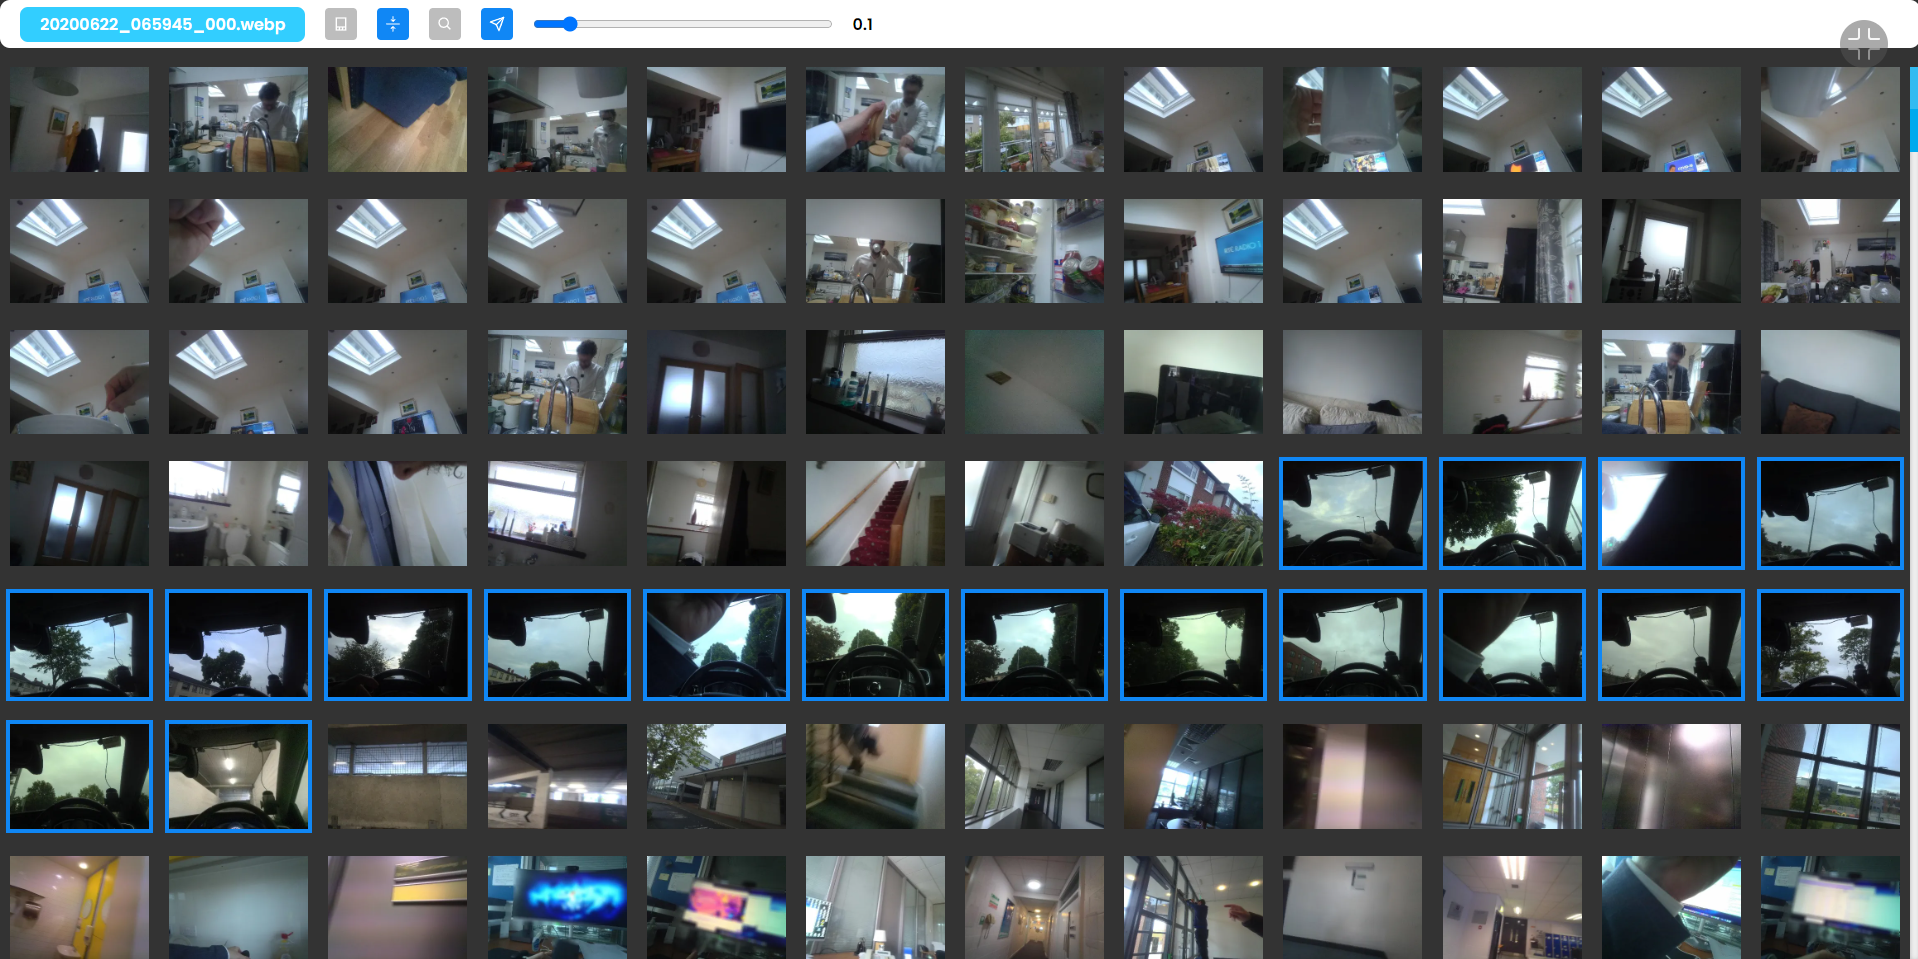
\includegraphics[width=0.9\textwidth]{content/resources/images/methods/FIRST_timeline_before.png}
    \caption{The interface of our Timeline View, gallery mode. }
    \label{fig:FIRST_timeline_before}
\end{figure}

\begin{figure}[H]
    \centering
    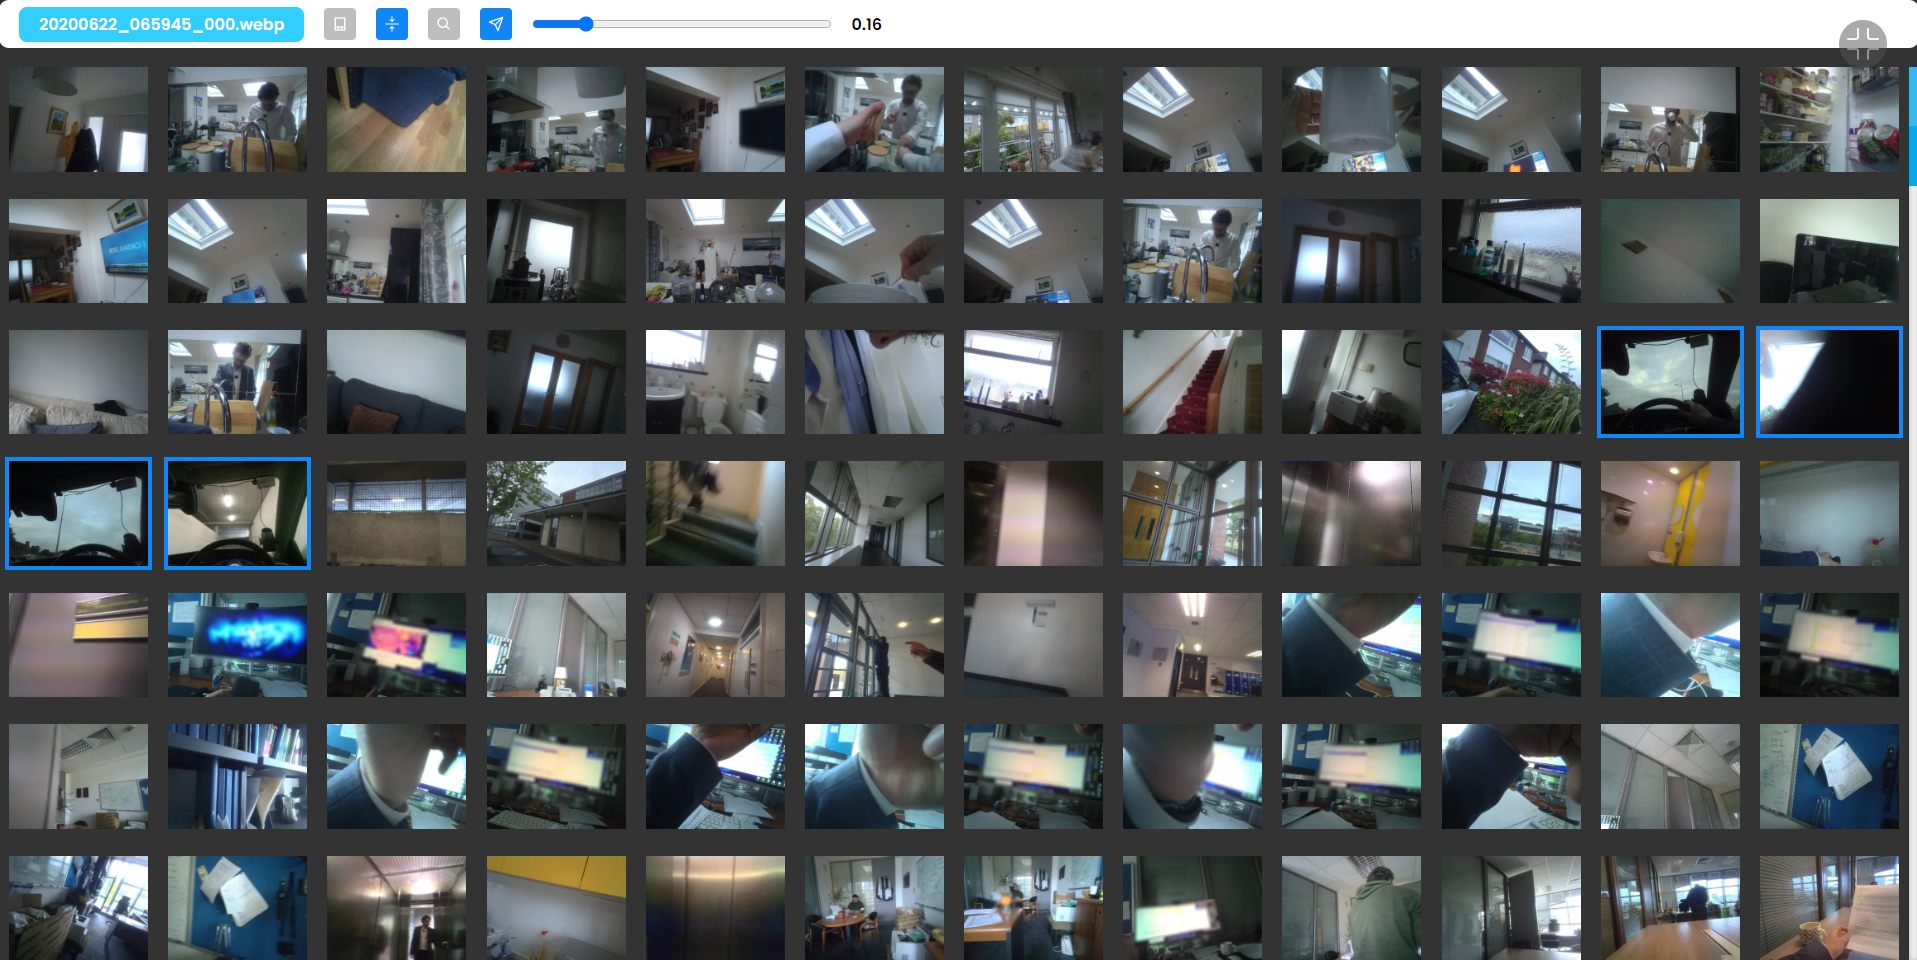
\includegraphics[width=0.9\textwidth]{content/resources/images/methods/FIRST_timeline_after.png}
    \caption{The interface of our Timeline View, gallery mode, with a higher threshold (more concise) than Figure \ref{fig:FIRST_timeline_before}.}
    \label{fig:FIRST_timeline_after}
\end{figure}

\section{Back-end design}
\label{sec:first_back_end_design}

\begin{figure}[h]
    \centering
    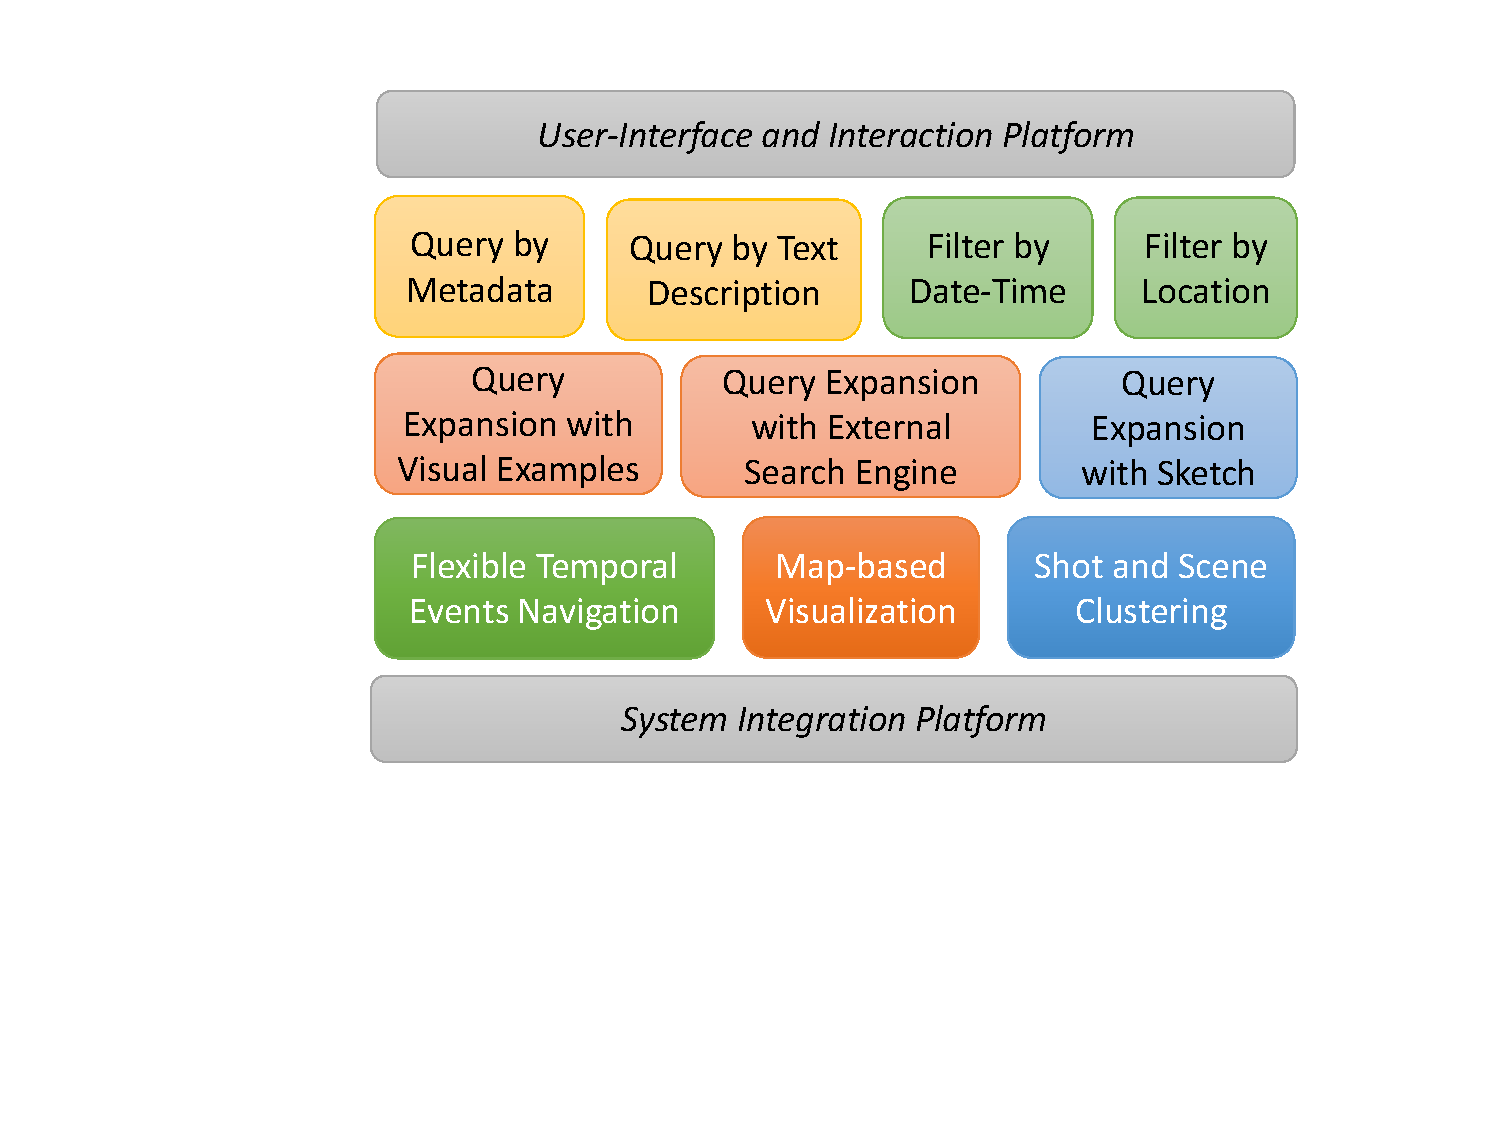
\includegraphics[width=0.8\textwidth]{content/resources/images/methods/FIRST3Components.pdf}
    \caption{Overview of the components of our system.}
    \label{fig:retrieval_components}
\end{figure}

Figure \ref{fig:retrieval_components} shows the overview of the various components in our system, which is developed from FIRST 2.0 \cite{trang-trung_flexible_2021}. The top and bottom layers are platforms on which we can integrate our modules for operational and visualization purposes.

\vspace{-2mm}
\subsection{Efficient clustering of data}
\label{sec:clustering_data}

\vspace{-2mm}
As lifelogging data is periodically taken from the wearable camera every few seconds, they are equivalent to uniform sampling from a video. When dealing with sampled images of this kind, there are a lot of similar-looking images, as the lifelogger cannot always be moving. This phenomenon can be confirmed by looking at Figure \ref{fig:FIRST_timeline_before}, where it can be observed that in a single day, there are lots of consecutive images that are relatively indistinguishable. This is the same situation with videos, as they cannot rapidly introduce new content. Processing the data as-it will result in enormous work with little helpful outcome. For videos, this problem is called the keyframe detection problem, which is challenging on its own. As lifelogging data is not dense enough compared to regular videos (1-2 FPS vs 30 FPS) and spans a much longer time (1 day vs a few minutes), directly applying key frame detection to lifelogging data will be difficult. While coarser sampling can be a quick fix, it can significantly hurt recall, for additional sampling will result in information loss when the sampling is already scarce. 

Besides storage issues, having similar images with no additional information will cause great trouble during retrieval. When an image is deemed relevant, obviously similar images will also be considered such; however since we only return the \textit{top-k} retrieval results, the result will contain many clusters of similar images, which would significantly reduce the variety of the returned results, hindering searching.

We propose a simple grouping strategy to deal with similar images by leveraging the strong expression capability of the visual embedding model used \cite{radford_learning_2021}. We consider images in chronological order and group two consecutive images if their distance in the embedding space is less than a pre-defined threshold. Chains of consecutive grouped images will form \textit{shots}, which we represent with only one image (e.g., the first one) of the shot and discard the rest. This strategy is relatively \textit{safe}, as it only removes very similar-looking images while still preserving slight changes in a small region (e.g., the lifelogger is watching TV), therefore we can be assured that it results in almost no information loss. Though it does not entirely solve the problem, the information density has already increased exceptionally, as we could exclude nearly $30\%$ of the images in the LSC'22 dataset from the vector database using this method with a conservative threshold. 

\vspace{-2mm}
\subsection{Temporal navigation with varying level of details}
\label{sec:temporal_navigation}

\vspace{-2mm}
When we find a relevant image, there is a realistic need to check the preceding/succeeding images to see if the content of the segment agrees with the single image. Some teams seek to implement a feature that allows \textit{playing} the video that contains said image. However, we note that this feature puts a heavy burden on the network and is also not fast enough (the user has to wait for the video to play). Instead, we propose to keep the gallery view and augment it by developing the idea proposed in Section \ref{sec:clustering_data}. While in Section \ref{sec:clustering_data} we cluster the data as a pre-processing step to reduce the amount of data in the vector database, we can simultaneously apply it to shrink the gallery of each day, allowing fast browsing through it and effective usage of screen space compared to the video playing approach. To completely negate the need to view the original data, we need to have varying levels of details, on one side, the user can summarize the sequence to as few as a dozen images, while on the other end of the spectrum, the user can choose to view the original data as-is. Note that even in the latter case, the system only needs to handle all the images in a single day, therefore it still allows for better organization and optimization of data storage. The interface of this feature is depicted in Section \ref{sec:timeline_view}.

\subsection{Attention-based embedding enrichment}
\label{sec:attention_based_embedding_enrichment}

A traditional approach for lifelog retrieval is to extract concepts from an image so that it can be indexed. The extracted concepts can be entities appearing in the image, type of place, type of action, etc. However, this approach depends on the concept detectors for known concepts in a pre-defined dictionary. Therefore, this method is inappropriate for searching for new concepts unavailable in that dictionary.


Keeping in mind the openness of our retrieval system, we aim to represent an image with feature vectors that can be used to match with new concepts. 
For each image in the dataset, we extract a high-dimensional representation using CLIP \cite{radford_learning_2021}. This embedding is a good general descriptor of the image and is close to its main features (concepts). In this way, our system can support users search for simple concepts related to entities in an image (such as \textit{chair}, \textit{TV}, \textit{sandwich}, \textit{etc}) as well as more abstraction concepts (such as \textit{a lecture class}, \textit{a wedding ceremony}, \textit{etc}).

However, the lifelogging data contains very similar scenes in which a subtle change in the image's content can differentiate one image from hundreds of similar ones (e.g., the content of the TV at that time). Therefore, apart from the general concepts in the image, we are also interested in more subtle and local features. 

\begin{figure}[t]
    \centering
    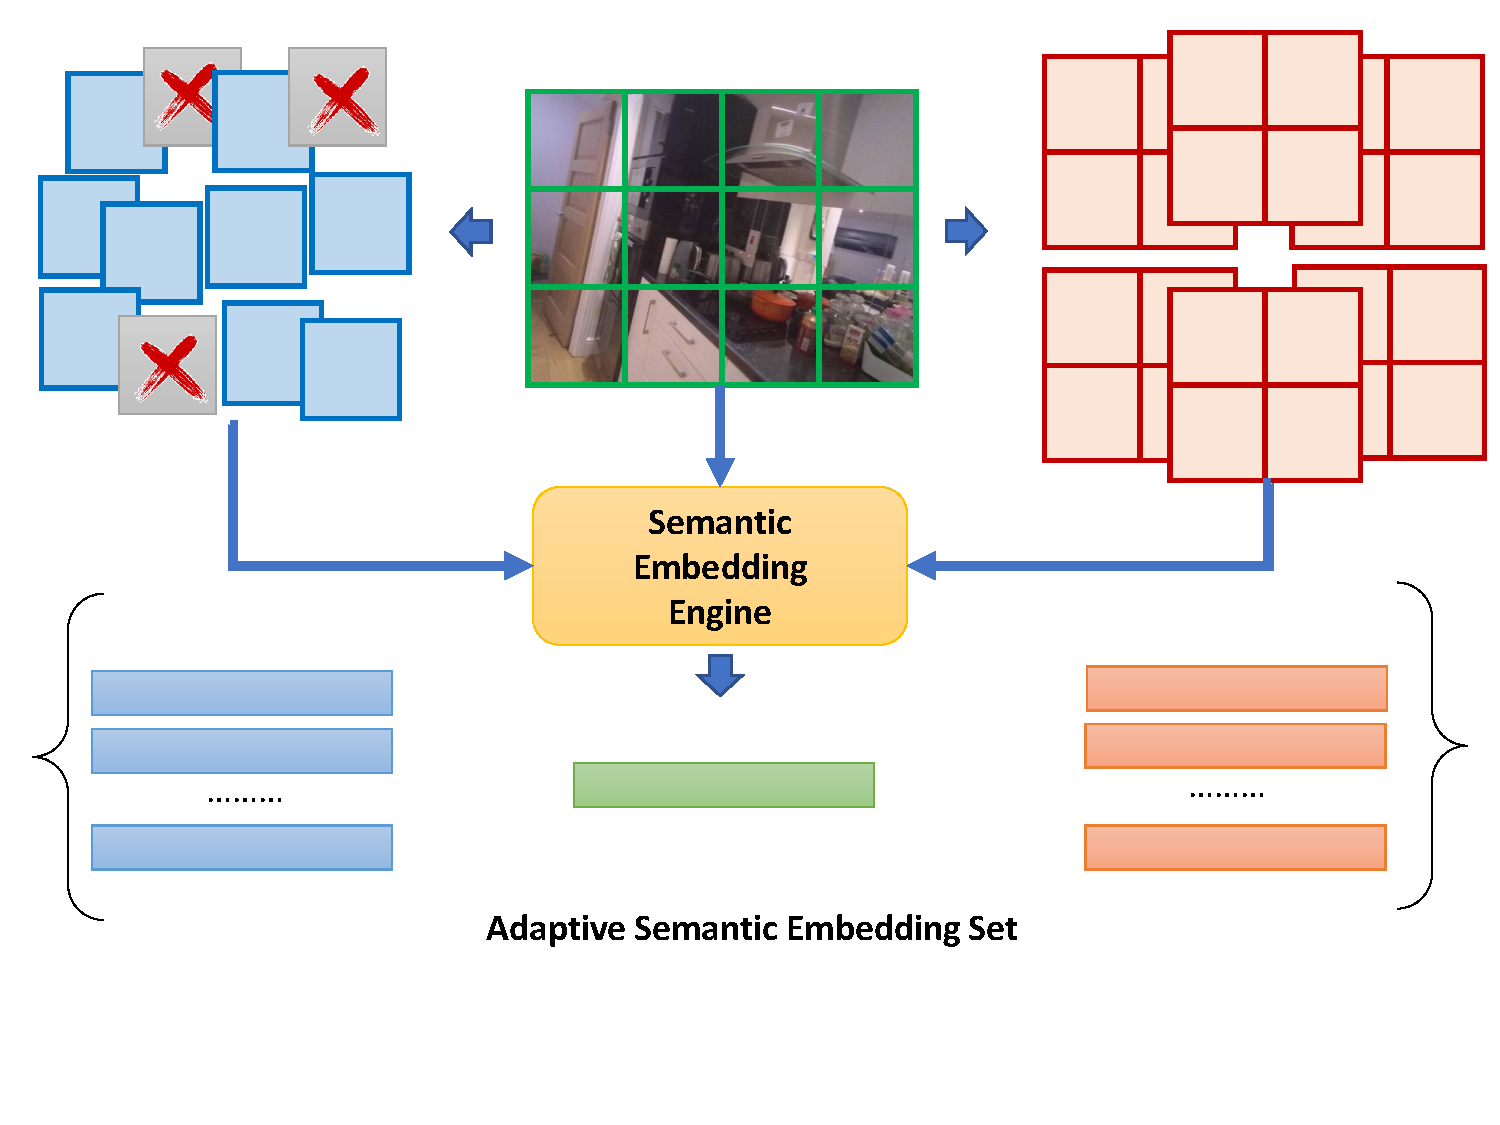
\includegraphics[width=1\columnwidth]{content/resources/images/methods/AdaptiveSemanticEmbeddingSet.pdf}
    \caption{Image decomposition and Adaptive semantic embedding set.}
    \label{fig:AdaptiveSemanticEmbeddingSet}
\end{figure}


Furthermore, since the original size of the images is $1024 \times 768$ and the CLIP model encodes images of size $224 \times 224$ or $336 \times 336$ depending on the model used, they have to be down-sampled in order to be encoded by CLIP, which can cause loss of information. Furthermore, it would not be sufficient to query, \textit{i.e.} to match, an object or concept appearing in a small portion of an image from the global embedding vector of that image. Hence, it should be necessary to encode various important regions of an image at different levels of detail to assist in retrieving different concepts at various levels of granularity in an image.

Due to the above reasons, we seek to add additional information besides the overall image embedding. To achieve this, we select smaller crops of the image and encode them along with the original image. This is similar to the attention mechanic in that we focus on "interesting" regions in the image. The regions to be selected are usually the ones that contain salient objects that can define the scene. This way, we can represent an image with an adaptive semantic embedding set.

Figure \ref{fig:AdaptiveSemanticEmbeddingSet} demonstrates our idea to decompose an image into multiple patches corresponding to different levels of detail and generate an adaptive semantic embedding set corresponding to that image. In our implementation for FIRST 3.0 \citeown{hoang-xuan_flexible_2022}, for simplicity, we represent an image (with the aspect ratio of 4:3) as a grid with $4 \times 3$ square cells. Then we construct multiple patches with the size of $1 \times 1$ and $2 \times 2$ cells, which can be overlapped. Finally, we remove unimportant patches and encode information-rich patches into semantic embedding vectors. The adaptive semantic embedding set is the collection of semantic embedding vectors of the full-size image and its exciting patches.

\subsection{Visually similar image searching}

As stated in Section \ref{sec:first_system_design} in the principle of \textit{Openness}, we use similarity modelling to extend the capabilities of our system. This is a feature that many other methods also seek due to its usefulness in the retrieval setting \cite{nguyen_lifeseeker_2022} \cite{lokoc_enhanced_2021}. In our system, we leverage the strong representational capability of CLIP \cite{radford_learning_2021}, which is demonstrated to be effective even in the zero-shot setting \cite{portillo-quintero_straightforward_2021}. Because CLIP was trained on image-caption classification task, which is a form of contrastive training, we believe it has learned to differentiate between images based on the concepts existing in the images, and so it can encode the image regardless of the content. More importantly, this allows us to simply define the distance between two images as the cosine distance between their embeddings. With this definition, we can quickly find an image similar to a given image in a database. This gives rise to the ability to search using visual examples.

In multiple cases, there are some concepts that cannot be well described using words, are unknown to the user, or are unavailable in the training corpus for the text encoder. Such instances are present in previous editions of the LSC. While trying to expand the pre-defined dictionary helps in all cases, it requires much effort to identify the needed concepts and also comes with storage and computing costs. We deviate from this paradigm by two means: utilizing \textit{external} systems and modelling \textit{deep} image semantic.


\begin{figure}[]
    \centering
    \vspace{-2mm}
    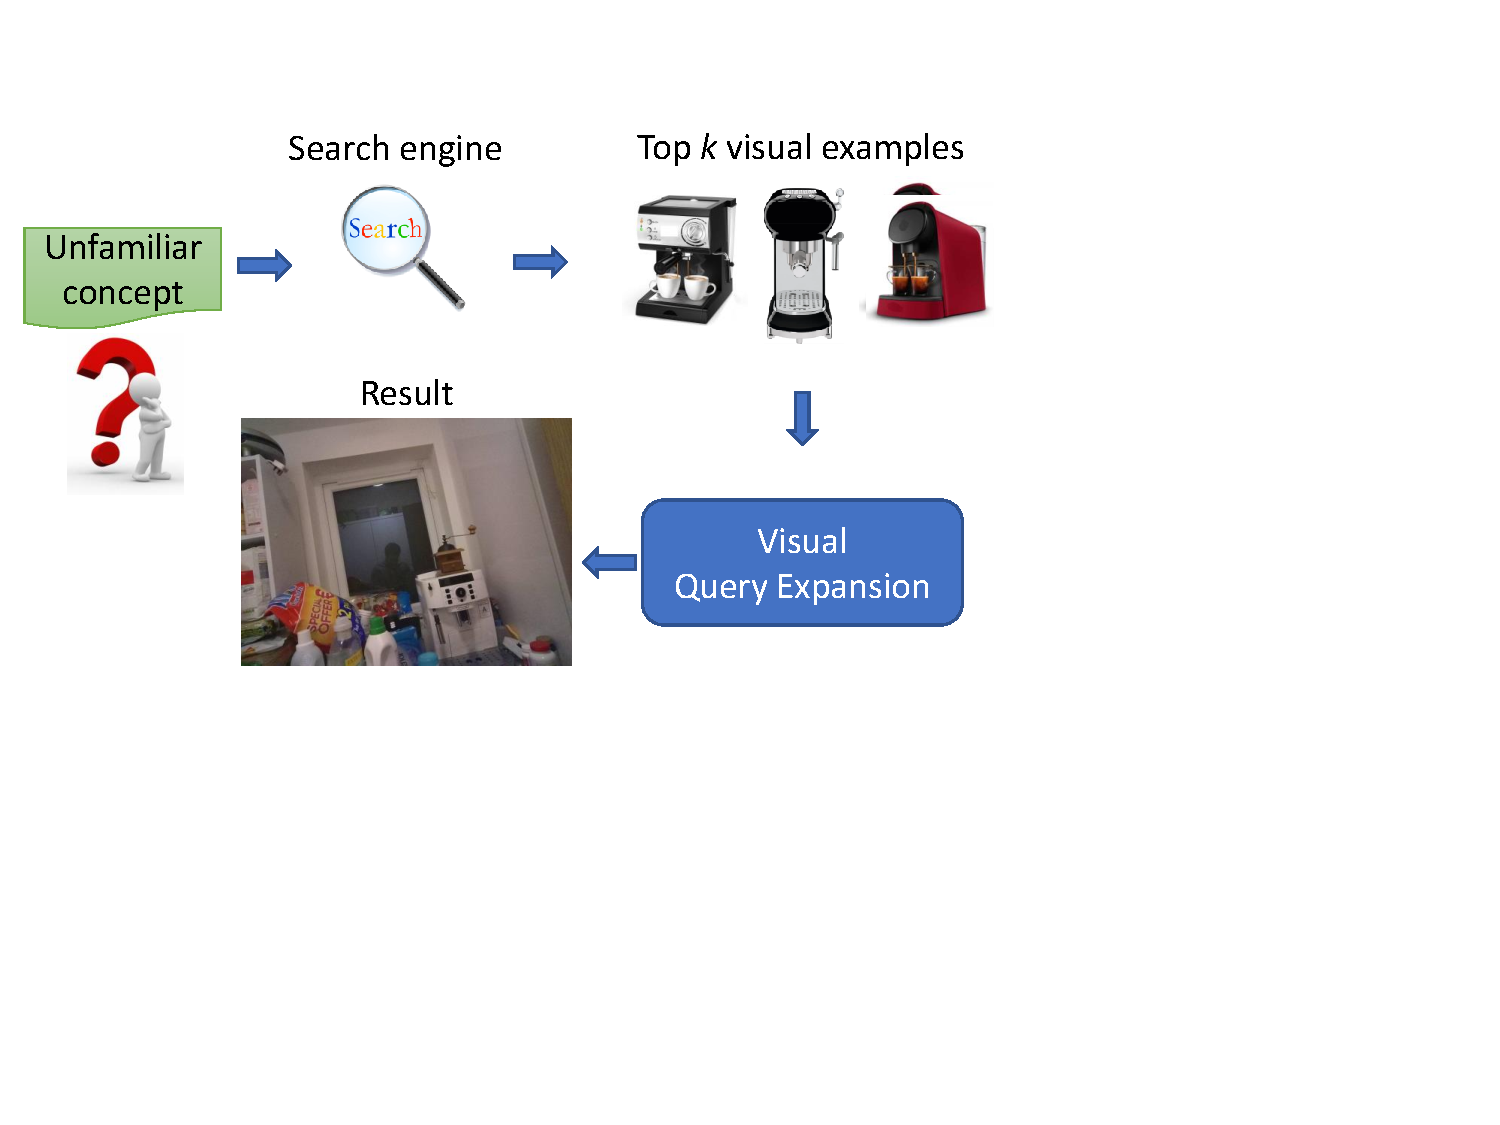
\includegraphics[width=0.9\columnwidth]{content/resources/images/methods/VisualQueryExpansion.pdf}
    \caption{Retrieval of an unfamiliar concept with the assistance of visual search engine.}
    \label{fig:VisualQueryExpansion}
\end{figure}

With the ubiquitous amount of data available on the Internet, we believe that any possible concept, possibly along with an image-text correspondence, exists and can be found with an appropriate tool, such as Google Search. We can query those tools to find an example of such a concept and use it as a starting point for our retrieval process. With our visual comparison capabilities mentioned earlier, we support the use of an external image as a prototype for query, as demonstrated in Figure \ref{fig:VisualQueryExpansion}. We can look for \textit{coffee machine} with visual examples suggested by an external search engine. This approach allows us to broaden the scope of searching beyond our existing concepts and utilize the strengths of other systems while producing a natural and intuitive searching process. This feature works well with our adaptive embedding described in Section  \ref{sec:attention_based_embedding_enrichment}, as the particular unknown/unfamiliar concept usually only occupies a portion, or even a tiny bit of an image, and therefore focusing on it greatly helps with "matching" it to the available prototype.

Many works \cite{tran_e-mysce_2022}, \cite{trang-trung_flexible_2021} enrich images with metadata tags from pre-trained state-of-the-art object detectors. While this is intuitive and effective, and we do this ourselves too, we propose a further advancement by modelling more abstract concepts from the image, such as events. This can be achieved in a number of ways, one of them is breaking down or associating an abstract concept with simple concepts or objects that can be searched for. An example of this is that instead of searching for "teaching", which is difficult to define, we can try to look for whiteboards, people in a room, desks, etc. As another avenue, we note that recent advances in representation learning have made this more possible than ever; we show that since CLIP was trained on image-caption pairs, it has some (limited) ability to understand a scene in the same way a human does. We can directly leverage this to empower our searches. By leveraging general representations instead of task-specific representations, advances to these models also empower our search engine without intervention. We believe this direction may prove useful and make future search engines simpler yet more powerful.

% \subsection{Query expansion via pseudo relevance feedback}

\section{Lifelog Search Challenge 2022}

The Lifelog Search Challenge (LSC) provides an opportunity for developers to qualitatively and quantitatively benchmark their system, both through expert and novice users, on a common dataset in a common setting. It has been organized every year since 2018 as an offline workshop, with the exception of 2020 and 2021 due to the COVID-19 pandemic. By gathering all systems and evaluating on the same dataset and queries, it is possible to benchmark the performance of different systems fairly. Furthermore, the assembly also facilitates the exchange of ideas and discussion of problems and potential solutions, gradually improving the quality of participating systems and the challenge as a whole.

In its 5th iteration, the LSC'22 was held in a hybrid format in Newark, New Jersey, as part of the ACM International Conference on Multimedia Retrieval (ACM ICMR'22). Our participation was online due to difficulties in applying for a U.S. visa.

\subsection{Dataset}

The LSC'22 dataset is recorded by a lifelogger using a wearable camera 24/7. The dataset consists of approximately 750000 images, spanning a time period of 18 months, and taking up storage of 44 GB. The dataset is fully anonymized and redacted before publication: faces and sensitive texts were identified and blurred, while sensitive scenes were filtered and deleted. 

\subsection{Query format}

The search topics are divided into 3 categories for LSC'22:

% And finally, since everyone has taken part in a testing session, we all know the query types, but just to remind everyone:
% - KIS Topics - Find one relevant item from the collection to match the temporally increasing query. Total time is 5 minutes. Standard VBS / LSC KIS scoring is used here which penalises incorrect submissions. These are automatically judged against a pre-calculated list of correct items. If there is a dispute over a topic, we can evaluate a disputed item after the topic (in the competition).
% - Ad-Hoc Topics - Find as many relevant items as possible with a 3 minute time period. Each of these have to be judged in real-time, so these will take time if a lot of submissions are made.  For VBS participants, this is similar to the textual AVS task.
% - Q&A Topics - The idea here is to find one correct answer to the topic. You are only allowed to submit one answer, which will be judged correct or incorrect. There is a 3 minute time limit on this type of topic. This is scored as a KIS task, so time to find the item is important.

\begin{itemize}
    \item \textbf{Known item search (KIS)} - This topic requires participants to find the one relevant image from the collection. Participants will be given a textual description of the item, and more clues will be gradually revealed over a period of 5 minutes. The scoring will be based on how soon the team finds it and the number of incorrect submissions. 
    \item \textbf{Ad-hoc topics (AD)} - This topic demands as many relevant items as possible within 3 minutes. Unlike KIS, the topics are usually much broader (e.g., "find all images of toy trains"). Since there can be diverse answers, the submissions are judged manually.
    \item \textbf{Question answering (QA)} - Originating from the need of automatic question answering systems, this topic allows only a single submission to address a particular information need (e.g., "what is my house's number?"). The submitted image should explicitly contain this information, and it will also be manually judged.
\end{itemize}

One of the actual queries for LSC'22 was: \textit{I think it was the second time I visited a stone shed. The shed was under green trees. It takes 2 hours to drive there and 2 hours back. It was in May 2020.} The answer can be found in Figure \ref{fig:LSCsample}. As can be seen, the prompt consists of multiple sentences, each shown gradually one after another, each revealing additional information (\textit{stone shed}, \textit{under green trees}, \textit{driving}, \textit{date}). The participant has to selectively combine all of this information to locate the answer in the shortest time possible.

\begin{figure}[h]
    \centering
    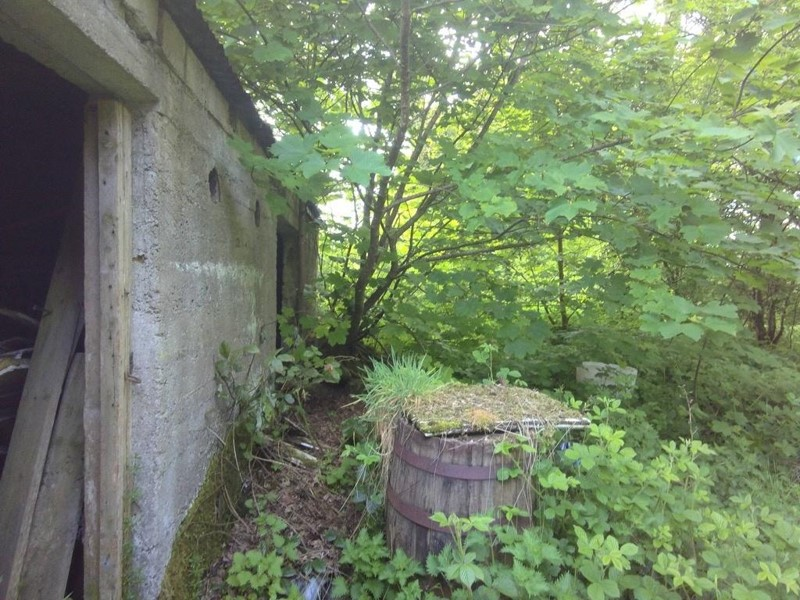
\includegraphics[width=0.6\textwidth]{content/resources/images/evaluation/LSCsample.jpg}
    \caption{Sample answer for an actual query at LSC'22.}
    \label{fig:LSCsample}
\end{figure}

\vspace{-2mm}
\subsection{Evaluation method}

\vspace{-2mm}
For the LSC, one of the judges, who is also the lifelogger that records the dataset, will generate queries based on their memory. Teams will be tested on a (possibly uneven) number of topics of all three categories during the workshop session, in no particular order. 

\vspace{-2mm}
The participants will view the queries and submit their answers via the DRES system. The scores will be separate for each category, with the final score being the sum of each category. Within each category, the scores are normalized such that the top performing team's score is always 100. The particular scoring functions for KIS and ad-hoc topics are different, and QA topics are judged as KIS topics.



\section{Visual Browser Showdown 2022}

The Video Browser Showdown (VBS) is a long-time video search competition with the goal of developing fast and effective video search systems. It has a very similar format to the LSC; in fact, it is the LSC that is based on the VBS competition as it has been around since 2012 as part of the International Conference in Multimedia Modeling (MMM). The VBS works with general video data, unlike the LSC, which is focused on lifelogging. Many teams participate in both VBS and LSC because they are similar in format, and at the same time, each competition presents a different challenge that they can evaluate their system on.

For the 2022 edition, the Visual Browser Showdown 2022 (VBS 2022) challenge was held in Phu Quoc, Vietnam, in conjunction with MMM 2022. While the conference was held in a hybrid format, we took the chance to participate on-site.

\subsection{Dataset}

The VBS competition shares the same dataset with TRECVID (\textbf{T}ext \textbf{RE}trieval \textbf{C}onference \textbf{VID}eo Retrieval Evaluation), a workshop sponsored by the National Institute of Standards and Technology (NIST) also working information retrieval research. The dataset used for VBS 2022 is V3C1 and V3C2 combined, which amounts to 17235 videos, totalling approximately 2300 hours and 3 TB of storage. The dataset is based on Vimeo, an online video-sharing platform similar to YouTube.

\subsection{Query format}

VBS 2022 features very similar search topics to LSC'22, with minor differences. Note that VBS works with video data, therefore the search target for KIS tasks is a short segment (usually under a minute) of a video that contains the event(s) described by the prompt.

\begin{itemize}
    \item \textbf{Known item search - Text (KIS-T)} - This topic is the same as LSC known item search. However, since the VBS data is not lifelogging data, the description is focused on the people, objects, and scenes present in the video, without information such as time.
    \item \textbf{Known item search - Video (KIS-V)} - For this topic, a short segment of a video is given, and participants are asked to locate it (i.e., find the video id and its timestamp). Everything else is the same as KIS-T tasks. 
    \item \textbf{Ad-hoc topics (AVS)} - This topic demands as many relevant items as possible within the time limit. Note that in this topic (and all other topics), image submissions are expected.
\end{itemize}

\subsection{Evaluation method}

The queries are generated by the judges prior to the competition, as with LSC. Scores are separately normalized for each category, and the overall result is the sum of each category.

\section{Interactive Retrieval Results}

We report the benchmarks of our system from LSC and VBS competition, in addition to detailed analysis of overall performance and case study. From experience we gained during the development and actual usage of the system, we sum up some best practices for novice and intermediate users to make the most of our system.

\subsection{LSC'22}
\label{sec:LSC22}

\begin{figure}[h]
    \centering
    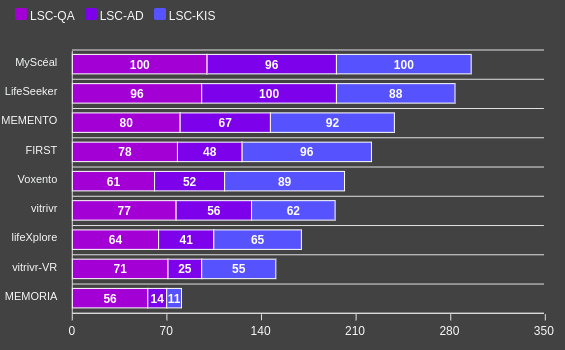
\includegraphics[width=\textwidth]{content/resources/images/evaluation/LSC2022_results.png}
    \caption{Result of all teams at LSC'22. Our team's name is FIRST.}
    \label{fig:LSC2022_results}
\end{figure}

At LSC'22, we placed 4/9, winning Best KIS (after overall winner MyScéal). The breakdown of all categories for all teams can be found in Fig \ref{fig:LSC2022_results}.

As our system is designed with KIS in mind, overall, our system performs best within that category. QA is a new category that requires ancillary tools (e.g., a map), while AD tasks require detailed processing of the original videos.

\subsection{VBS 2022}
\label{sec:VBS2022}

\begin{figure}[h]
    \centering
    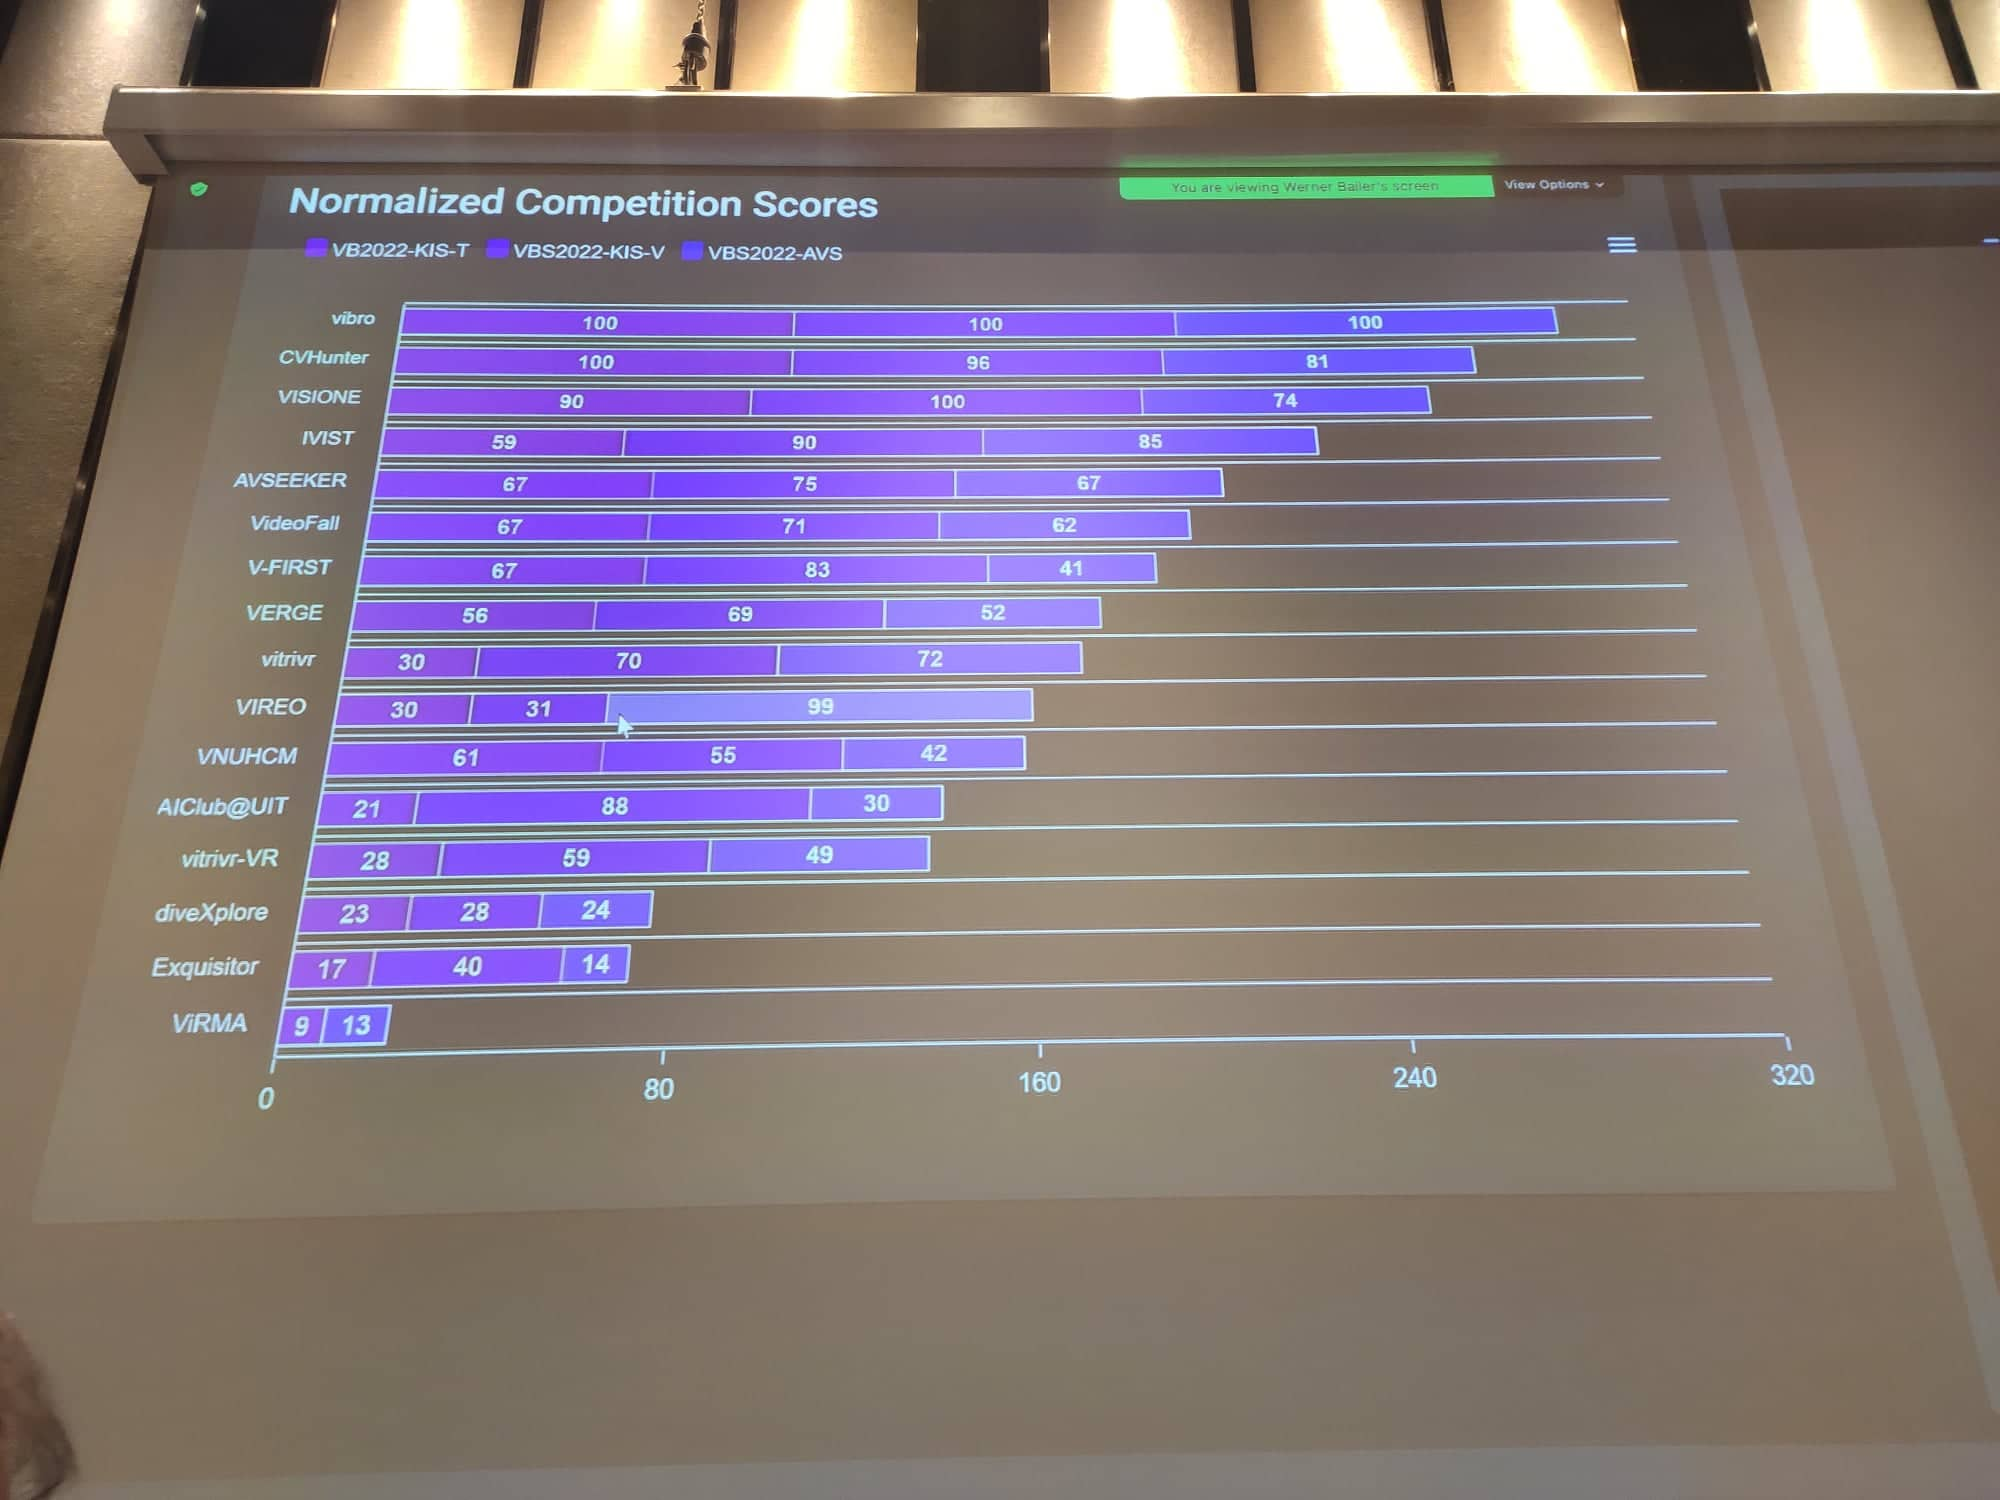
\includegraphics[width=\textwidth]{content/resources/images/evaluation/VBS2022_results.jpg}
    \caption{Result of all teams at VBS2022. Our team's name is V-FIRST.}
    \label{fig:VBS2022_results}
\end{figure}

At VBS 2022 \citeown{tran_v-first_2022}, we placed 7/16, just a bit behind Best Newcomer VideoFall. We scored 67 on KIS-T, 83 on KIS-V, and 41 on AVS. The detailed results can be seen in Fig \ref{fig:VBS2022_results}.

\subsection{Case study}
\label{sec:CaseStudy}

% 1: removal of repetitive scenes allow for varied results: lighting fixture 
% 2: focus on local content: TV content
% 3: image searching: pendant lamp


% example: 20190101_140454_000

\vspace{2mm}

In this section, we describe some specific usage scenario to demonstrate how to best use our system, as well as its strengths.



\textbf{Scenario 1:} \textit{I was looking at a lead soldier in a mall, next to some clothes.}

We think of two strategies to approach this query, either directly searching for "\textit{lead soldier}", or imagining a typical lead soldier and trying to describe it. For the second strategy, we might attempt to look for a standing man, wearing a red shirt and a top hat. 



\begin{figure}[h]
    \centering
    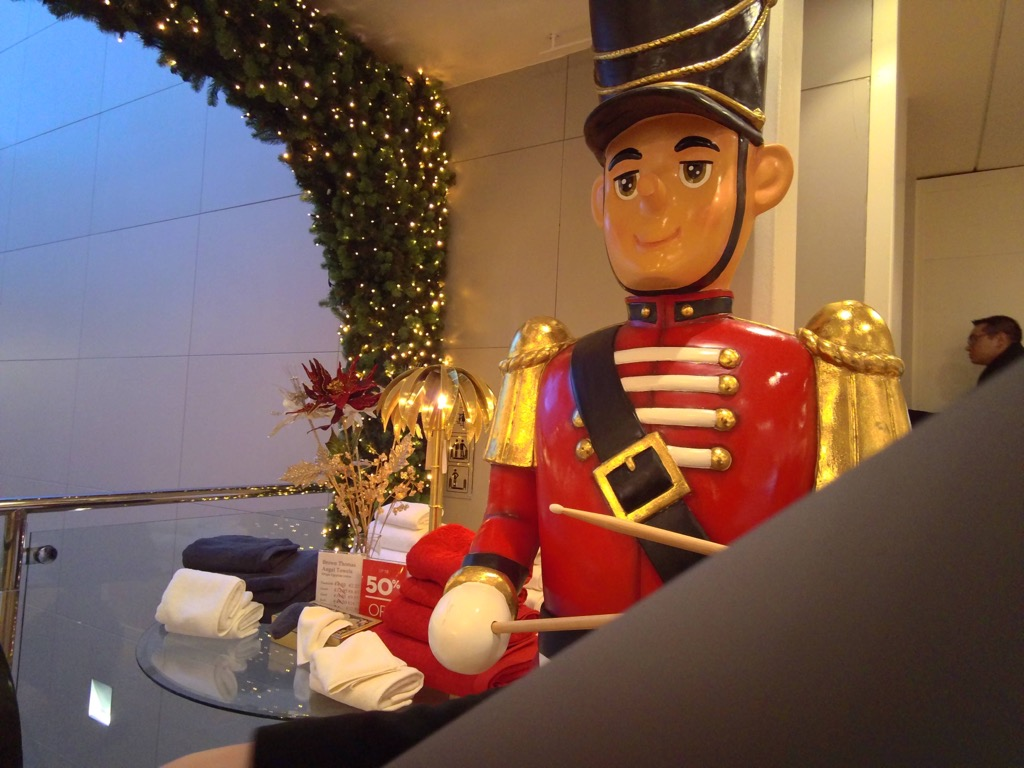
\includegraphics[width=0.7\columnwidth]{content/resources/images/methods/CaseStudy1Target.jpg}
    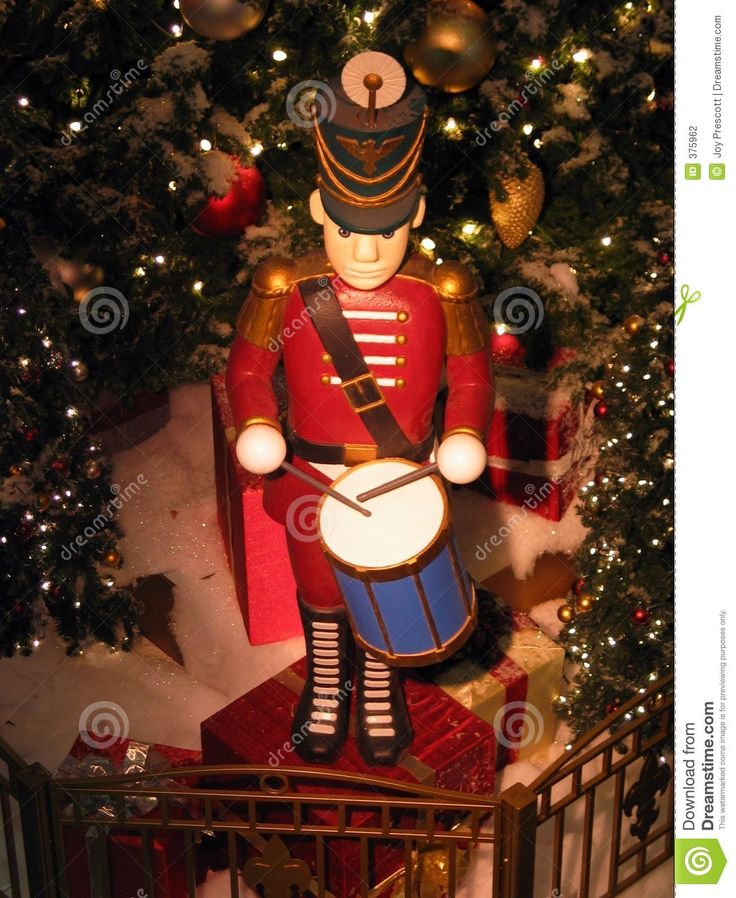
\includegraphics[width=0.25\columnwidth]{content/resources/images/methods/CaseStudy1Prototype.jpg}
    \caption{The first scenario. The target image is on the left, while the image on the right is the prototype we took from Pinterest.}
    \label{fig:CaseStudy1}
\end{figure}

The results of both approaches are shown below.
\begin{itemize}
  \item[] a lead soldier standing \xmark
  \item[] a lead soldier wearing red shirt \xmark
  \item[] a lead soldier wearing red suit \cmark
  \item[] a man wearing red suit \xmark
\end{itemize}



We observe that searching for "man" or "red suit" yields too many results and not the one we are looking for, and even in the query that successfully found the target image, the results are inconsistent. Instead, we can search for a concrete example on the Internet and use it directly for our search, as shown in Figure \ref{fig:CaseStudy1}. This gives the target image as the top-2, and at the same time, yields two other images with a lead soldier in it in the top-15, which none of the shown queries was able to. As mentioned above, we only need the URL of the image, so the process is fairly quick and much faster than the try-and-error approach of query engineering.




\textbf{Scenario 2:} \textit{I was taking a photo of a man sitting at a table. I took a flight to this city 3 days ago. I was in Greece then.}

\vspace{-2mm}
In this example, we would like to illustrate our system's capability to retrieve a moment with the activity or story in an image, instead of looking for only entities/objects appearing in it. With the first sentence in the query description, rather than looking for the moment when we can see a smartphone or camera in a photo, we can simply search with the text description "\textit{I was taking a photo of a man sitting at a table}". 

\vspace{-2mm}
If there are multiple moments, we can verify the event of interest using the second sentence in the query. Three days can be a long duration and it would be inconvenient and inefficient for a user to navigate through a long sequence of images just to verify the previous event of taking flight and arriving at a new city. Our system assists users with a flexible navigation mechanism and grouping similar images into shots, thus the system helps users quickly confirm the moment happening 3 days ago. 

\begin{figure}[t]
    \centering
    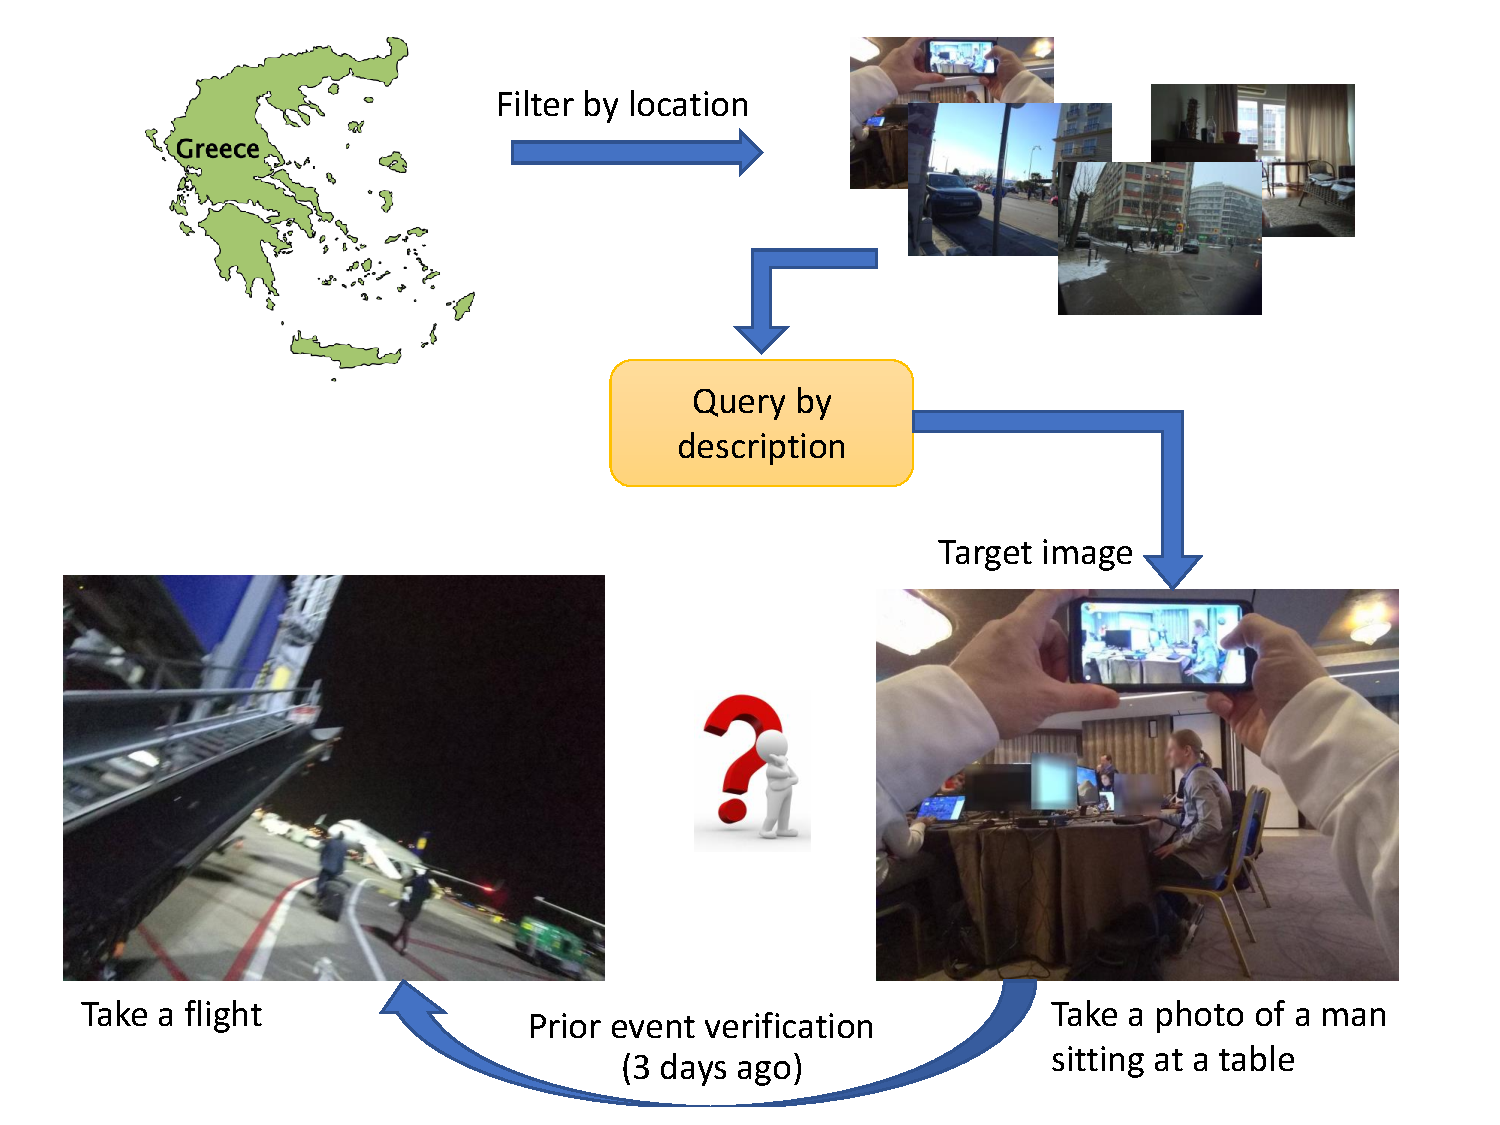
\includegraphics[width=1\columnwidth]{content/resources/images/methods/CaseStudy2Overview.pdf}
    \caption{The second scenario. The target image can be identified from description, location filtering, and prior event verification.}
    \label{fig:CaseStudy2}
\end{figure}

\vspace{-2mm} 
Finally, if we wait until the last minute to exploit the last sentence in the query description, we can narrow down the moments occurring in Greece. We can simply set the filter on the location ("\textit{in Greece}") and query with the description from the first sentence, and we can successfully identify the target moment, as illustrated in Figure \ref{fig:CaseStudy2}.

\textbf{Scenario 3:} \textit{I was in a shop, talking to a woman in front of some purses. One of them was purple and the other one was white.}

\begin{figure}[t]
    \centering
    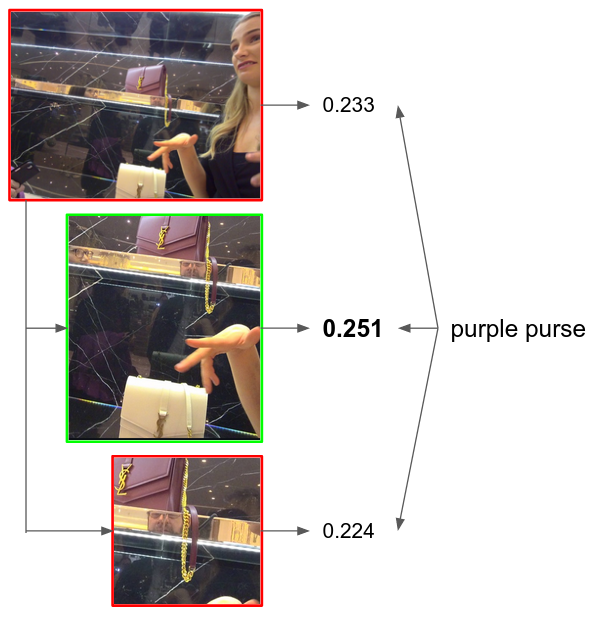
\includegraphics[width=0.7\columnwidth]{content/resources/images/methods/CaseStudy3Overview.png}
    \caption{The third scenario. The target image is shown at the top, following by a $2 \times 2$ patch and a $1 \times 1$ patch containing the purse. The images are not scaled equally. }
    \label{fig:CaseStudy3}
\end{figure}

\vspace{-2mm}
For this query, we could try to locate the shop through geolocating or finding other shopping moments and browse for a fashion shop that sells purses. We believe that there are few images of a purple purse, so we focus on this hint. However, from the description, we know that the purse does not occupy the whole image, this can make it difficult to find it if we only encode the whole image. 

Indeed, the local features mentioned in section \ref{sec:attention_based_embedding_enrichment} help us in this case, as the correct crop can better highlight the purse. Note that the varying sizes matter, as the $1 \times 1$ patches fail to capture the purse, and only the $2 \times 2$ patch is able to fully capture it. Being able to centralize on the purse while ignoring other objects pushes it closer to the "purse" concept and allows it to be found. The scenario is depicted in Figure \ref{fig:CaseStudy3}. The scores represent in the figure are the similarity (higher is better) to the query phrase "\textit{purple purse}". In this case, only the $2 \times 2$ patch is close enough to make it to the top results, the other images are too far down the ranklist. 


\subsection{Best practices}
\label{sec:best_practices}

Due to many factors, novice users (i.e., people that are not familiar with retrieval systems and/or do not have knowledge of the underlying model/data) have difficulty operating the system with performance that is comparable to expert users or system developers. In our work \citeown{hoang-xuan_flexible_nodate}, we propose to devise a few guidelines on which users can create their own strategy to use when searching. The idea for this proposal is based on the fact that in the challenges/competition, the systems are operated by developers who have a good understanding of the system, therefore they are extremely proficient when searching. The reason for this is that through extensive testing, they have become used to the scenarios that are usually presented with during the competition, and they know exactly which tools are best to overcome each obstacle. We believe this knowledge can be summed up and explained to normal users without requiring a precise understanding of the underlying system. This is especially beneficial as it dramatically improves the average performance and usefulness of the system without needing any modifications.

With all said, the compiled list of best practices is as follows:

\begin{enumerate}
    \item \textbf{Maximize specificity} \quad In a given prompt, there can be multiple concepts and objects that are being referred to. It is wise to choose the concept that is most unique to the search target since it will quickly reduce the number of possible candidates, or in terms of information theory, choose the concept that will maximize \textbf{information gain}.
    
    Example: suppose the prompt is asking for a picture of "a collection of phones, an Ipad, a wallet, and a vase on a table", it is pragmatic to look for an Ipad instead of a phone or a table. 
    
    For LSC tasks, the accompanying metadata (time, location, etc.) is especially useful here as they all help to very quickly narrow down the possible answers and should be applied almost automatically. 
    
    \item \textbf{Apply creativity} \quad More often than not, there are multiple ways to describe a single image. The differences come from word choice (simple vs advanced English), concept choice (abstract vs concrete), perception (e.g., pink vs purple), and more. Therefore, when one approach does not yield satisfactory result, it is imperative to try other avenues.
    
    Example: "a party on the beach" can also be described as "people with food on the beach", "person with plates next to sand and water", etc. 
    
    \item \textbf{Utilize visual similarity} \quad As popular search engines use text input, ordinary users are used to it. However, our system provides other means of searching as well. We emphasize the usage of visual search, as it is intuitive and easy to use yet often neglected. This feature works especially well with Ad-hoc topics. In some cases, there can be concepts that are hard to define using language, therefore an external visual example can also be used.
    
    Example: "salt lamp" is a concept that is under-represented in the data used to train the model joint-embedding model, but its visual example is sufficiently unique to search.
    
    \item \textbf{Do temporal verification} \quad People have a tendency to describe multiple moments in succession rather than a single one. This provides valuable information that can be used to distinguish the right moment from similar ones. Therefore, when dealing with multiple events, the Timeline View feature should be used to check whether the preceding/succeeding events follow the same narration. 
\end{enumerate}